\section{Transistor MOSFET(Metal-Oxide Semiconductor Field Effect Transistor)}

\begin{figure}[H]
    \centering
    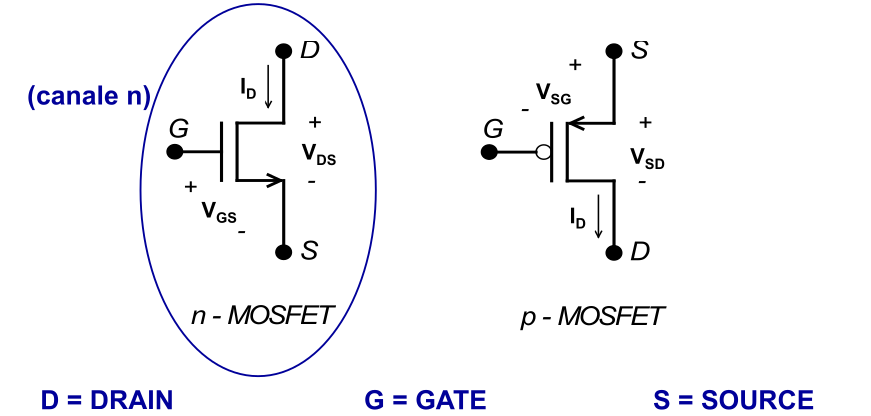
\includegraphics[width=0.5\linewidth]{2 - dispositivi elettronici/imgs/Screenshot from 2022-06-14 23-25-50.png}
\label{fig:MOSFET}
\caption{MOSFET}
\end{figure}

\subsection{Capacità MOS: accumulazione}

\begin{figure}[H]
    \centering
    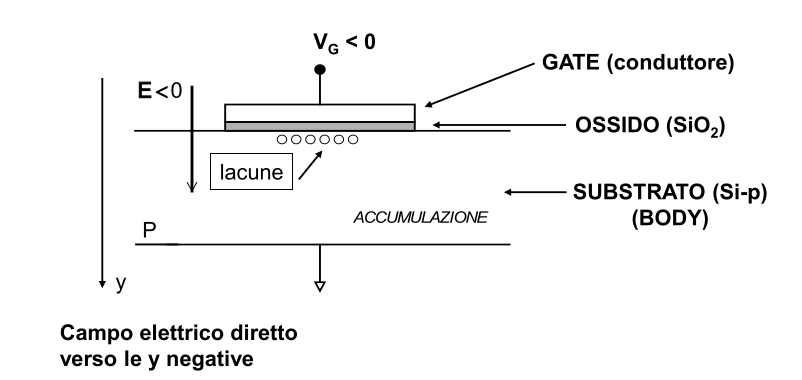
\includegraphics[width=0.5\linewidth]{2 - dispositivi elettronici/imgs/Screenshot from 2022-06-15 11-23-56.png}
    \caption{MOS accumulazione}
    \label{fig:MOS_acc}
\end{figure}

L'accumulazione è l'aumento di concentrazione di lacune sotto l'ossido del gate.

\subsection{Capacità MOS: svuotamento}

\begin{figure}[H]
    \centering
    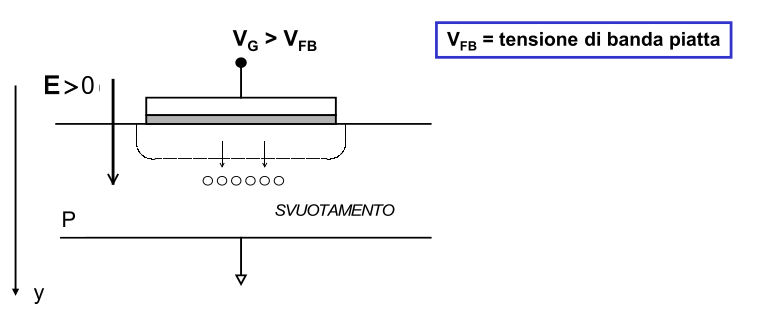
\includegraphics[]{2 - dispositivi elettronici/imgs/Screenshot from 2022-06-15 11-30-59.png}
    \label{fig:MOS_svuotamento}
    \caption{MOS svuotamento}
\end{figure}

Le lacune vengono allontanate dal campo elettrico e viene 
creata una zona svuotata sotto l'ossido del gate.